\documentclass{article}

\newif\ifdraft
% During writing: a draft:
%\drafttrue
% FINAL:
\draftfalse

\ifdraft  %% generate tableofcontents down to the \paragraph
\setcounter{tocdepth}{5}
\fi
%1. introduction
%        a) a statistician's needs
%        b) statistical analysis packages supported by ESS
%2. emacs 
%        a) buffers
%        b) key-binding
%        c) modes
%                1) font-lock
%                2) shell/comint
%                3) ange-ftp/EFS/tramp
%                4) vc/pcl-cvs
%3. ESS
%        a) interactive
%           1) S family
%           2) SAS
%        b) batch
%           1) SAS
%           2) BUGS
%           3) S family
%4. ESS as an open source project
%        a) origins
%                1)S-mode
%                2)SAS-mode
%        b) unification
%                1)ESS-mode
%                2)Emacs/XEmacs
%                3)Unix/Windows/Mac
%5. conclusion
%        a) summary
%        b) what's next for ESS
%   ESS internet resources
%        a) home page
%        b) ess-help
%        c) anonymous cvs
%   References
%
\ifdraft
 \addtolength{\topmargin}{-1cm}
 \addtolength{\textheight}{+1cm}
\else%FINAL:
 \renewcommand{\baselinestretch}{1.5}
\fi
\addtolength{\oddsidemargin}{-0.5in}
\addtolength{\textheight}{0.2in}
\addtolength{\textwidth}{1in}

%%%
\usepackage[authoryear,round]{natbib}
%or (if you have an unshiny latex installation)
%\newcommand{\citep}[1]{{\{\sf#1\}}}
%%%
\usepackage{alltt}

%% Postscript fonts
\usepackage{times}
\usepackage{graphicx}
%\usepackage{psfig}

\ifx\pdfoutput\undefined
  %% Stuff wout hyperref
  \def\url#1{\stexttt{#1}} % To help fit in lines ?AJR: stextsf?
\else
  %% Stuff with hyperref
  \usepackage{hyperref}
  %%\hypersetup{backref,colorlinks=true,pagebackref=true,hyperindex=true}
  \hypersetup{backref,colorlinks=false,pagebackref=true,hyperindex=true}
\fi
%%---End of package requiring ---------- Own Definitions -------------

\newcommand*{\regstrd}{$^{\mbox{\scriptsize{\textregistered}}}$}
\newcommand*{\tm}{$^{\mbox{\scriptsize\sc tm}}$}
\newcommand*{\SAS}{\textsc{SAS}}
\newcommand*{\Splus}{\textsc{S-Plus}}
\newcommand*{\XLispStat}{\textsc{XLispStat}}
\newcommand*{\Stata}{\textsc{Stata}}
\newcommand*{\Rgui}{\textsc{Rgui}}
\newcommand*{\Perl}{\textsc{Perl}}
\newcommand*{\Fortran}{\textsc{Fortran}}
\newcommand*{\Scmt}[1]{\hbox{\qquad {\footnotesize \#\#} \textsl{#1}}}
\newtheorem{defn}{Definition}[section]
\newtheorem{ex}{Example}[section]

\newcommand{\stexttt}[1]{{\small\texttt{#1}}}
\newcommand{\ssf}[1]{{\small\sf{#1}}}
\newcommand{\elcode}[1]{\\{\stexttt{\hspace*{2em} #1}}\\}
\newcommand{\file}[1]{`\stexttt{#1}'}
\newcommand{\US}{{\char'137}}        % \tt _
\newcommand{\marpar}[1]{\marginpar{\raggedright#1}}
\newenvironment{Salltt}{\small\begin{alltt}}{\end{alltt}}

\newcommand{\emptyfig}{
\hspace*{42pt}\rule{324pt}{.25pt}\\
\hspace*{42pt}\rule{.25pt}{10pc}
\rule{316pt}{.25pt}
\rule{.25pt}{10pc}}

%% Use \begin{Comment} .. \end{Comment} for internal comments
\ifdraft
\newenvironment{Comment}{\begin{quote}\small\itshape }{\end{quote}}
%
\else  %% this requires
  \usepackage{verbatim}
  \let\Comment=\comment
  \let\endComment=\endcomment
\fi


%%--------------------------------------------------------------- Start Text

\title{Emacs Speaks Statistics (ESS): A multi-platform, multi-package
intelligent environment for statistical analysis}

\author{A.J. Rossini \and Martin M{\"a}chler \and Kurt Hornik \and Richard
  M. Heiberger \and Rodney Sparapani \footnote{%
%%
    A.J. Rossini is Research Assistant Professor in the Department of
    Biostatistics, University of Washington and Joint Assistant Member at
    the Fred Hutchinson Cancer Research Center, Seattle, WA, USA
    (E-mail: rossini@u.washington.edu);
%%
    Martin M{\"a}chler is Senior Scientist and Lecturer in the Seminar for
    Statistics, ETH Zurich, Zurich, Switzerland
    (E-mail: maechler@stat.math.ethz.ch);
%%
    Kurt Hornik is Professor in the Institut f{\"u}r Statistik,
    Wirtschaftsuniversit{\"a}t Wien and the Institut f{\"u}r
    Wahrscheinlichkeitstheorie und Statistik, Technische Universit{\"a}t
    Wien, Vienna, Austria (E-mail: Kurt.Hornik@r-project.org);
%%
    Richard M. Heiberger is Professor in the Department of Statistics at
    Temple University, Philadelphia, PA, USA (E-mail: rmh@temple.edu);
%%
    Rodney Sparapani is Senior Biostatistician in the Center for Patient
    Care and Outcomes Research at the Medical College of Wisconsin, 
    Milwaukee, WI, USA (E-mail: rsparapa@mcw.edu)}}

%%S\date{\today}
\date{$ $Date: 2002/02/15 17:31:46 $ - $Revision: 1.177 $ $\tiny printed \today}

\begin{document}

%%\ifpdf
%%  \DeclareGraphicsExtensions{.jpg,.pdf,.png,.mps}
%%\fi
%%%% To cite everything
%%\nocite{*} 

\ifdraft
\setcounter{page}{0}
%%\newpage
\tableofcontents
\fi

\maketitle

\ifdraft{}%% large line skip -- please not yet (MM)
\else%FINAL:
 \renewcommand{\baselinestretch}{1.5}
 %%- \baselineskip=2pc
\fi

\begin{abstract}
  Computer programming, both using statistical packages and writing
  them, is an important component of statistics research and data
  analysis.  Emacs Speaks Statistics (ESS) provides an intelligent,
  consistent interface between the user and the software.  ESS
  interfaces with SAS, S-PLUS, R, and other statistics packages under
  the Unix, Microsoft Windows, and Macintosh operating systems.  ESS
  is itself a package within the Emacs text editor and uses Emacs
  features to streamline the creation and use of statistical software.
  ESS knows the syntax and grammar of each data analysis package it
  works with and provides consistent display and editing features
  across packages based on that knowledge.  ESS assists in the
  interactive or batch execution by the statistics packages of
  statements written in their languages.  Each statistics package is
  run as a subprocess within the Emacs environment allowing the user
  to work directly from the editor and therefore retain the
  consistency of always being in the same environment.  We discuss how
  ESS works and how it increases statistical programming efficiency.
\end{abstract}

\noindent Keywords: Data Analysis, Programming, 
S, \SAS, \Splus, R, \XLispStat, \Stata, BUGS, free-software,
open-source, cross-platform

\section{Introduction}
\label{sec:introduction}

Most statistical research activities, particularly data analysis and
communication, involve some form of computing.  The computer user
interface is thus placed in the central role of facilitating
statistical tasks.  While presentation of character and graphical
%of components, information, and similar output 
information is the most visual component of a user interface,
perhaps a more critical component is how the computer interprets user
input.  A familiar, well-understood set of input behaviors can provide
large gains in efficiency.  This paper introduces Emacs Speaks
Statistics (ESS) \citep{ESS}, a software package which provides a
common interface to a variety of statistical packages on the most
common computing platforms.

ESS is a statistical package interface which provides, through Emacs,
tools which facilitate both statistical software development and data
analysis.  ESS provides assistance with both writing and evaluation of
analysis code for both interactive and batch statistical
packages.  ESS currently supports the S family of languages (including
S \citep{BecRCW88,ChaJH92,ChaJ98}, \Splus\regstrd\ \citep{Splus}, and
R \citep{ihak:gent:1996}); \SAS\regstrd\ \citep{SAS:8}; \XLispStat\ 
\citep{Tier90} and its extensions Arc \citep{Cook:Weisberg:1999} and
ViSta \citep{youn:fald:mcfa:1992}; \Stata\ \citep{Stata:7.0}; Omegahat
\citep{DTLang:2000}; and BUGS \citep{BUGS}.  ESS can be extended to
accommodate most statistical packages which provide either an
interactive command-line or process batch files for instructions.

We start by describing the Emacs text editor, the underlying
platform on which ESS is built.  Next, we discuss how ESS enhances a
statistician's daily activities by presenting its features
and showing how it facilitates statistical computing.  The unique
history of ESS as an open source project follows; it is a
synthesis of several independent projects and has passed through 
generations of developers.  We conclude with future
extensions and related work.

\section{Emacs}
\label{sec:emacs}

Emacs is a mature, powerful, and extensible text editing system which
is freely available under the GNU General Public License (GPL) for a
large number of platforms, including most distributions of
Unix\regstrd, Microsoft Windows\regstrd\ and Apple Mac\tm\ OS.  There
are two open-source implementations of Emacs released
%which are released for use 
under the GPL: GNU Emacs \citep{GNU-Emacs} and XEmacs
\citep{XEmacs}.  Emacs shares many features with word processors, and
some characteristics with operating systems, including many facilities
which go beyond ordinary text editing.  More important to our goals,
Emacs can control and interact with other programs.

\paragraph{Keyboard and Mouse Input.}
When Emacs was originally written, character-based terminals were the
most advanced method of computer access.  Common Emacs commands were
mapped (or bound) to key sequences for convenience which are called
key-maps (or key-bindings).  Over the
last decade, Emacs has been extended to use graphical windowing
systems, such as X11\tm, Microsoft Windows, and Apple Mac OS, which
allow additional forms of input, for example using a mouse, and which
encourage multiple applications to share a single display.  Presently,
Emacs is more often used with a GUI, with commands bound to mouse
actions, but having commands also associated with key-maps
is an important time-saving feature so your hands don't have to leave 
the keyboard.
%for fast typists.
Emacs menus and toolbars on the display screen allow mouse access to
frequently used actions and provide a graphical alternative when the
user does not know or can not recall a key-binding; these are also
subject to user-customization.

\paragraph{Buffers give Emacs control.}
Emacs buffers are the interface between the user and computer.  They
can be considered to be a collection of scratch pads that both the
user and computer can read, write, and respond to.  The user can
simultaneously edit many files and control numerous programs by
initializing multiple buffers.  With disk files, the working copy of
the opened file is placed in an Emacs buffer where it can be viewed
and edited either by the user or automatically by Emacs or another
program under the control of Emacs.  Emacs will save a backup of the
contents to disk at specified intervals based on some function of time
and the amount of editing activity.  Emacs can present the buffers'
contents in ways which optimize the users reading and navigation
activities.  One program that is commonly run within Emacs buffers is
the interactive operating system command line interpreter, called a
shell.  By using this, most programs which take input from and provide
output to the command-line can run within and be controlled by Emacs.
The resulting buffer provides a copy of the entire transcript of the
interaction, which can be edited and searched during the program's
execution.

\paragraph{Major and Minor Modes.}
Emacs capabilities are extended by loading text files containing code
written in Emacs Lisp (elisp) \citep{RChassell1999}, a dialect of Lisp
\citep{PGraham:1996}.  Emacs commands, which are actually Lisp
functions, can be called interactively either by name or by pressing
their mapped key.  Not all functions are interactive in nature, and
only those that are can have key bindings.  The most important
extensions to Emacs are called modes, which can be major or minor,
depending on the extent to which they take over the editing behavior.

Major modes provide a customized environment consisting of mapped keys
and associated commands for editing a file or performing a task such
as reading mail or browsing disk directories.  Only one major mode can
be active for a given buffer at any time.  Major modes for file
editing are often determined by the file name extension, i.e. the
characters at the end of the file name that follow a period like
\stexttt{txt}, \stexttt{R} or \stexttt{sas}.  Examples of this kind of
major mode are \stexttt{ESS[S]} and \stexttt{ESS[SAS]}.  Major modes
know the syntax of their file type or application and therefore can
provide intelligent actions such as automatic indentation; navigation
in units of characters, words, lines, sentences, paragraphs, function
definitions, and pages; syntax-based fontification and colorization;
and reformatting based on programmed conventions.  Major modes also
provide the ability to perform tasks which are not specifically
text-editing.  They can interface with system programs to provide
command shells, read mail, and control other programs.

By contrast, minor modes provide services that are useful, perhaps
with a small amount of customization, for many major modes.  For
example, \stexttt{font-lock-mode} allows Emacs to highlight, with
fonts or colors, the syntax of a programming language whose
characteristics are described within a major mode like
\stexttt{ESS[S]}.  The \stexttt{overwrite-mode} determines whether
typed characters replace the existing text or are inserted at the
cursor.  Minor modes can be used to change key bindings to emulate the
keys used by another editor such as \stexttt{vi}.  In addition, they
can be used to perform version control operations and many other tasks
which are nearly identical across file types.

\paragraph{Network Support.}
Emacs allows transparent access to remote files over a network.
Transparent access means the user views, edits, and saves files on a
remote machine exactly as if they were on the local machine.
Mechanisms for both insecure (\stexttt{ange-ftp} and \stexttt{EFS} use
ftp) and secure (\stexttt{tramp} uses the secure shell protocol) are
available. The local Emacs can also monitor and control remote
processes running in a shell buffer.

\paragraph{Editing Extensions.}
Most programming and documentation tasks consist of editing text.
These tasks can be enhanced by contextual highlighting and recognition
of special reserved words appropriate to the programming language in
use.  In addition, Emacs also supports folding, outlining, and
bookmarks which can assist with maneuvering around a file.  Emacs
shares many features with word processing programs and cooperates with
markup language based document preparation systems such as \LaTeX,
\textsc{html}, or \textsc{xml}.

One feature which has only recently been incorporated into word
processors is the notion of flexible source code versioning.  Emacs
interacts with standard revision control programs such as CVS, RCS,
and SCCS through minor modes such as \stexttt{vc-mode}.  These
revision control systems facilitate documenting and tracking edits and
changes to a file.  More importantly, they allow for branching and
merging of versions so that material present in an older version of
the file can be recovered and inserted into a newer version in a
fairly easy manner.

Comparison of files, two or three drafts of a paper for example, is
simplified by \stexttt{ediff}.  An example is shown in Figure
\ref{f.ediff}.  The lines that are similar are highlighted in the two
buffers, one for each file, and the specific words that mismatch are
highlighted in a contrasting color.  \stexttt{ediff} has many tools
for working with the differences in files and in entire directories.
When combined with a source-code repository, it allows reinsertion of
deleted sections of code files, documentation, or papers.

\begin{figure}[tbp]
  \centering
  \ifdraft
     \emptyfig
  \else
     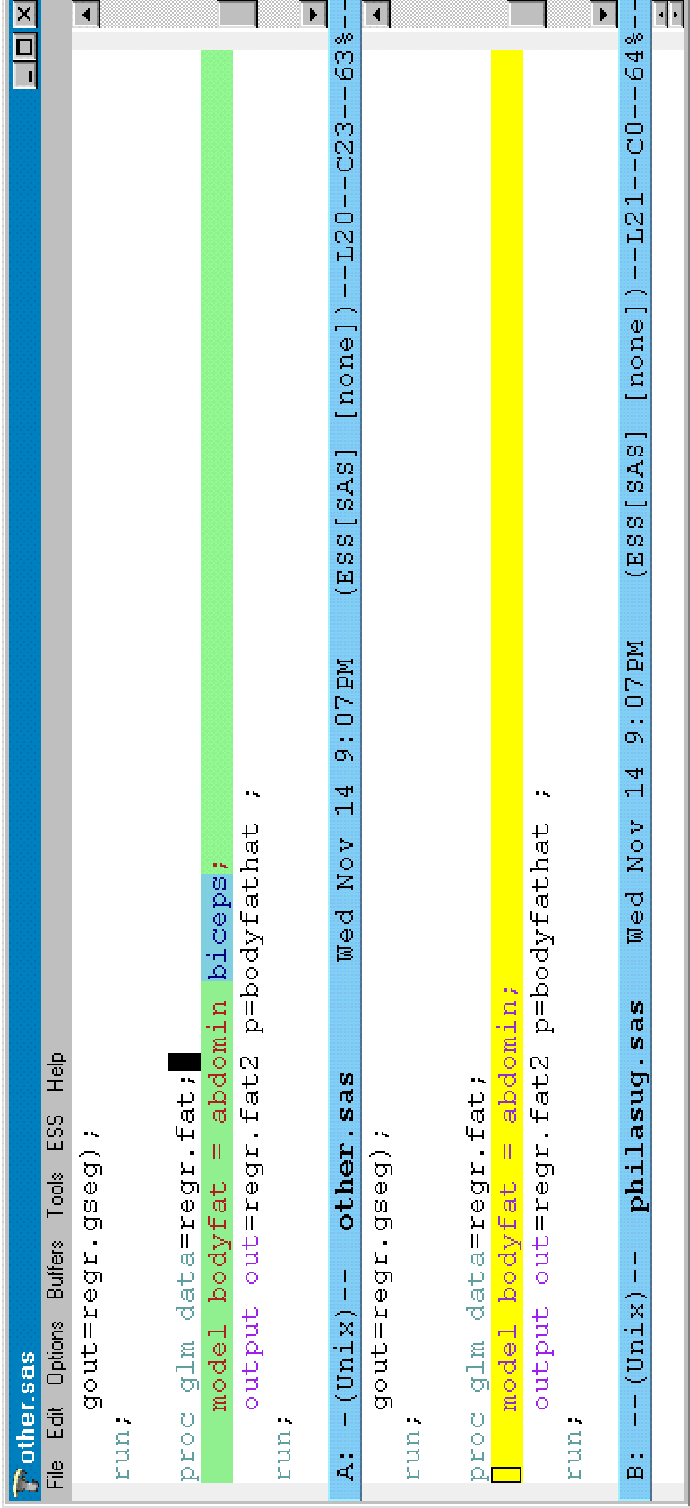
\includegraphics[angle=270,width=\textwidth]{ediff-sas}
  \fi
  \caption{Ediff of two versions of a file.}
  \label{f.ediff}
\end{figure}

There are many features which Emacs has which, while innovative when
introduced, are fairly common now.  Emacs provides file-manager
capabilities such as \stexttt{dired} (discussed in the Major and Minor
Modes paragraph above), which interfaces to the computer's directory
structure.  It also stores command-history records from the beginning
of an editing session, allowing a near-infinite undo capability.  More
importantly, for modes which control processes, the process input
history is stored.  The actual data analysis commands entered can be
very different from what is observed in the buffer after editing.
Tools such as \stexttt{etags} combined with \stexttt{speedbar} provide
a hyperlinked index to text objects, such as S function definitions
and \SAS\ \stexttt{PROC \dots\ RUN;} sections, across files within a
directory.  Other extensions to Emacs include web browsers, mail and
news readers, and spell checking.

Emacs is an extremely powerful editor.  Emacs has been claimed to
provide most of the capabilities found in an operating system.  This
provides a strong foundation for constructing an integrated
development environment which is focused on the needs of
statisticians.  Emacs' power, flexibility, portability, and
extensibility make it a solid platform on which to construct a
statistical analysis user interface.

\section{ESS extends Emacs}
\label{sec:ess-extends-emacs}

ESS extends Emacs to provide a functional and extensible interface
which is uniform and consistent across multiple statistical packages.
This is done by first, adding shortcuts and features for accelerated
editing of files, and second, by interacting with the particular
statistical packages through a number of activities: control of
input/output, assistance with evaluation, and specialized parsing of
help files.

Differences between user interfaces can arise from coordinating
several data files, multiple statistical software packages, and the
corresponding source code for each of these packages during a single
analysis.  ESS helps to remedy these differences by providing a single
point of contact for all tasks.  Other features, which are less
commonly employed by statisticians but provide potential for efficient
computer usage, include the use of version and source code control
systems, tools for accessing programs or files on remote machines, and
interfaces to documentation systems such as \LaTeX, presentation,
\textsc{html}, and \textsc{xml}.  Emacs can assist with, or be
programmed to perform, many tasks related to data cleaning,
management, and editing.  For example, conversion of data files
between standard input formats such as comma-separated or
tab-delimited can be automated fairly simply through the use of elisp
programs or keyboard macros.

% repetitive
%Below, we describe some of the
%problems that one encounters, and how ESS/Emacs can minimize the
%impact of the problems.

%This is done by extending the editor to provide
%additional useful features, and in the case of interactive statistical
%programs, sitting ``in front of'' their CLI and intercepting and
%modifying I/O as needed.  We describe the exact features more in this
%section.

%% change/edit
%Figure~\ref{fig:1} provides an example of how it looks when being used
%with XEmacs.  This screen-shot shows both SAS and R code being examined
%at the same time, with an R interactive process being controlled from
%within XEmacs.

%Figure~\ref{fig:2} shows ESS running in NTemacs 21.0 on Microsoft
%Windows 2000.  We are currently displaying 6 buffers.
%\stexttt{highlight.s} illustrates several uses of syntactic
%highlighting.  The most glaring one is the bright purple indicator for
%the unbalanced parentheses.  We also see color choices for keywords
%(\stexttt{if}), comments, and quoted strings.  The string on the last
%line was not properly terminated and we are immediately warned by the
%string color staying on through (what we think is) the end of the
%line.

%The two buffers \stexttt{transcript-before.st} and
%\stexttt{transcript-after.st} show transcript editing.  A single ESS
%command converted the before buffer into the after buffer by removing
%all lines that do not begin with a prompt character.

%The last three buffers show that a single S language source file can
%be used with two (or more) executing processes.  In this example we
%sent over first a subset of the line in \stexttt{tmps.s} and then the
%entire line to the instance of S+4 running in an inferior
%\stexttt{iESS(Sqpe)} buffer.  Then we switched the connection to send
%the same line to the instance of R running in the \stexttt{iESS(R)}
%buffer.  The dialog about the process switch appears in the message
%line.

\subsection{Features and capabilities}
\label{sec:ESS:features}

ESS fully supports the S family (S, \Splus, and R)\@.  \SAS\ and BUGS
are also well supported.  \Stata, \XLispStat\ (including extensions
ARC and ViSta) are supported with the basic functionality of syntax
highlighting and process-interfacing.  ESS and its interface are fully
discussed in the next section.

\paragraph{Syntactic highlighting and indentation of source code.}
The programmers task is eased when language constructs (such as
reserved words, function calls, strings, and comments) are visually
identifiable and when lines of code are automatically indented to a
depth appropriate to their context (e.g., if--then clauses, loops).
ESS provides both of these to the programmer by including a
description of the syntax of each supported statistical language in
the form used by \stexttt{font-lock-mode}.

Figure \ref{f.font} shows an example of font-locking a complicated S
statement.  The top panel shows an \stexttt{if} statement with a long
expression in the condition and a multi-line consequence.  The keyword
\stexttt{if} is shown in purple, the string \stexttt{"deltat"} in
RosyBrown.  The comments are in red.  Everything else is in the
standard font.  The consequence is indented and the continuations of
the consequence are further indented.  The matching parentheses are
shown in green.  The cursor is indicated by a solid box.  In the
bottom panel we replaced the matching parenthesis with an unbalanced
bracket.  Emacs immediately marks that with the paren-mismatch font,
bright purple in this example.  On a black and white terminal we would
use bold, underline, italic, and reverse-video, rather than colors, to
distinguish the fonts.

% Figure \ref{f.font} shows a black-and-white example of font-locking a
% complicated S statement.  The top panel shows an \stexttt{if}
% statement with a long expression in the condition and a multi-line
% consequence.  The keyword \stexttt{if} is shown in an underlined font,
% the string \stexttt{"deltat"} in an italic underlined font.  The
% comments are in an italic font.  Everything else is in the standard
% font.  The consequence is indented and the continuations of the
% consequence are further indented.  The matching parentheses are marked
% by a bold foreground and a shaded background.  The cursor is indicated
% by a solid box.  In the bottom panel we replaced the matching
% parenthesis with an unbalanced bracket.  Emacs immediately marks that
% with the paren-mismatch font, bright purple on
% a color terminal.

The font selection and the indentation depth are automatically
supplied by Emacs as the lines are typed.  The user has several
options for mapping of colors or fonts to each of the syntactic types.
We selected
%black-and-white font-mapping for display here.  On a terminal we might use 
purple for the keywords, red for comments, green for matching parens,
and inverse-video purple for mismatched parens.  Emacs makes default
choices of colors and ESS provides several other optional schemes.

\begin{figure}[tbp]%h
  \centering
\ifdraft
  \emptyfig
\else
  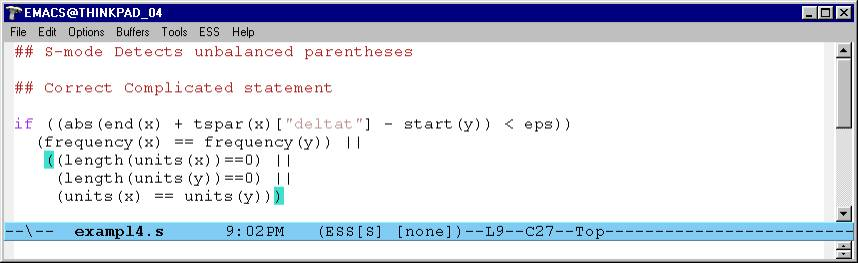
\includegraphics[angle=270,width=\textwidth]{font-cor-s}
  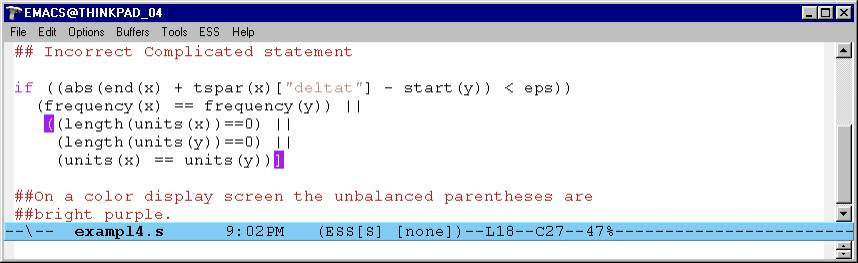
\includegraphics[angle=270,width=\textwidth]{font-incor-s}
\fi
  \caption{We illustrate here with fonts and colors appropriate for a
    color display.  On a black and white terminal we would use bold,
    underline, italic, and reverse-video.  On a color terminal we
    would use a selection of colors.}
  \label{f.font}
\end{figure}

For example, syntax highlighting can help enforce company coding
standards.  Figure \ref{f.hilock} shows how to enforce a standard for
\SAS\ programming that says all \stexttt{PROC} statements must use the
\stexttt{DATA=datasetname} option.

%\begin{Comment} Rodney: I agree that this is possible, however, I 
% have never seen a company attempt to enforce such standards.  In fact,
% I don't think it would be a good idea.  It would waste valuable time 
% checking SAS code that would be better spent verifying that the results 
% generated are correct (you have hit one of my pet peeves :o).
% I'd like to drop this controversial subject.  It makes us look like
% a bunch of auditors, rather than statisticians.

%Rich: This example was designed in response to an explicit request
%from the program chair of the Philadelphia SAS Users Group.  He felt
%that industrial SAS users were looking for this type of capability.
%The impression I got from him was that enforcement of standards was
%something that was wanted but that no one knew how to do.  The fact
%the Emacs can do it was a selling point.  It was very well received
%when I presented it at the meeting.

%Rodney: Having been a pharmaceutical SAS user from '93-'00, I can say
%that this is an improper use of auditing.  An auditors time is very 
%valuable and there are never enough auditors when you need them.  
%I'll give you an example.  We had to audit the CRFs of 2500 patients 
%in Europe and the auditors were embarking.  I wrote an undocumented, 
%not-following-the-standards SAS program to generate the audit sheets.  
%Instead of having them look at the code to see if it was compliant, 
%I sent them 50 audit sheets for patients that they already had the 
%source documents for.  As luck would have it, we had one patient that's 
%CRF did not match the audit sheet.  Further digging showed that the 
%Oracle database was not reporting the actual value that was in
%it's table due to a bug introduced in an upgrade 3 months earlier.
%Several hundred audit sheets that were already printed off were
%recycled and two people responsible for the Oracle database lost 
%their jobs.  This is the proper role of the auditor IMHO.  I think
%ESS should stay out of it, at least as far as the paper goes.
%\end{Comment}

\begin{figure}[tbp]
  \centering
  \ifdraft
     \emptyfig
  \else
     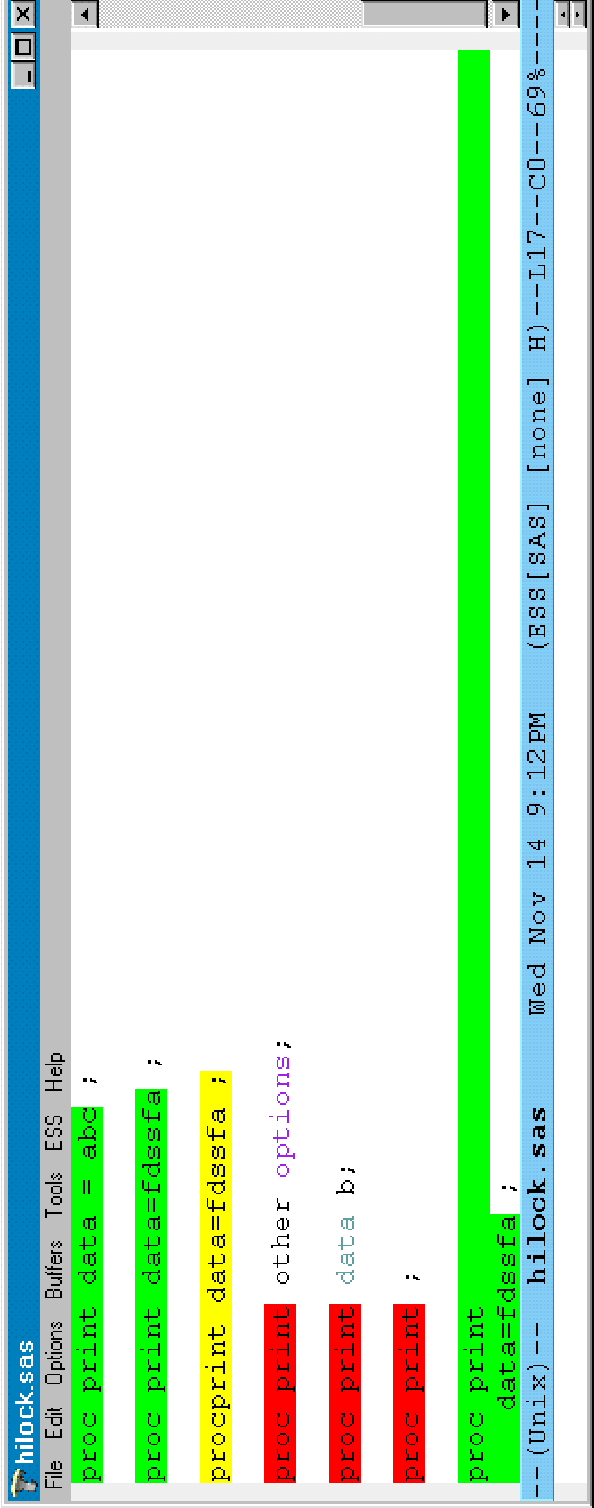
\includegraphics[angle=270,width=\textwidth]{hilock-sas}
  \fi
  \caption{Enforce company coding standards.  The standard here is
    that all \stexttt{PROC} statements must use the
    \stexttt{DATA=datasetname} option.  Lines that satisfy the
    standard turn green, lines that don't turn red.
    Ambiguous ones turn yellow.}
  \label{f.hilock}
\end{figure}

\paragraph{Process interaction.}
Emacs has historically referred to processes under its control as
``inferior'', accounting for the name inferior ESS (\stexttt{iESS}) to
denote the mode for interfacing with the statistical package.  Figure
\ref{f.ess-demo} shows the S language program \stexttt{ess-demo.s} in
the top buffer in \stexttt{ESS[S]} mode and the executing R process in
the bottom buffer \stexttt{*R*}.  The
(\stexttt{iESS}) major mode of the \stexttt{*R*} buffer is crafted for
command-line editing.  This mode remembers and uses the command
history, allowing for the recall and searching of previously entered
commands.  Filename completion for local directories is also
available.

\begin{figure}[tb] %p
  \centering
  \ifdraft
     \emptyfig
  \else
     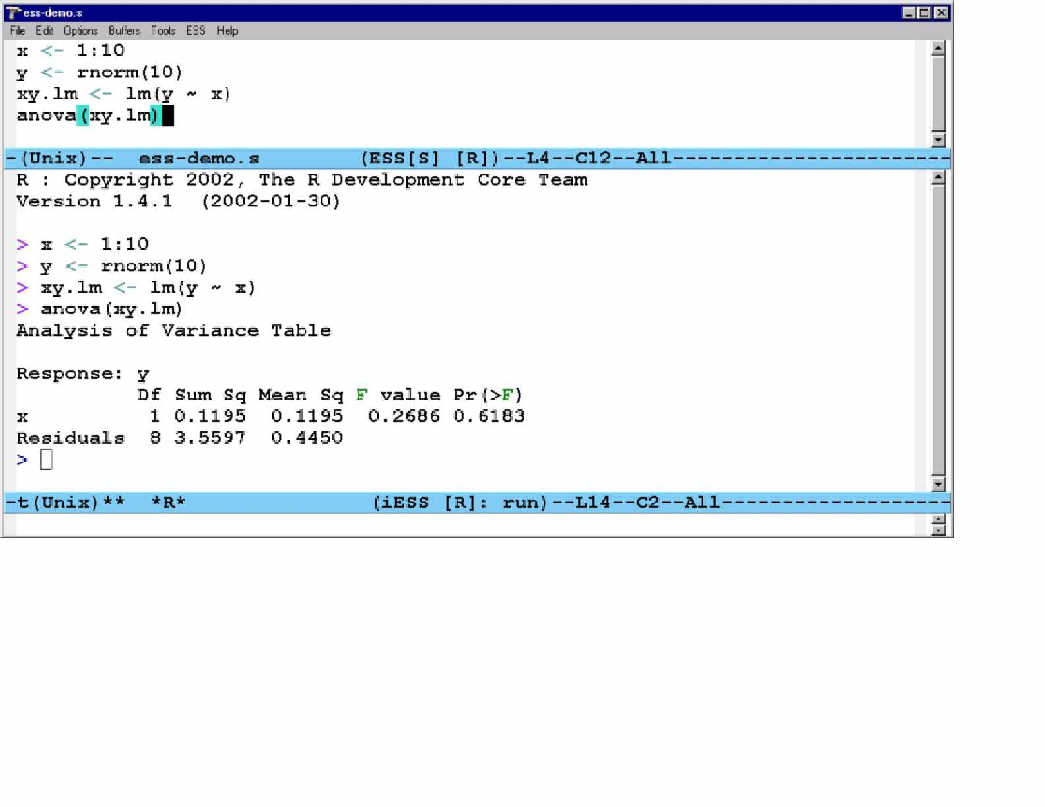
\includegraphics[angle=270,width=\textwidth]{ess-demo}
  \fi
  \caption{Line-by-line execution of a command file. The cursor is
    placed on a line in the \stexttt{ESS[S]} buffer and with a single
    keypress the line is sent to the \stexttt{*R*} buffer for
    execution.  The output of the package goes directly to the
    editable \stexttt{*R*} buffer.}
  \label{f.ess-demo}
\end{figure}

\paragraph{Source-level Debugging}
ESS facilitates the editing of source code files, sets of commands
written in the package's language by the statistical analyst, by
providing a means for loading and error-checking small sections of
code.  This is done through several mechanisms.  First, syntactic
highlighting of code makes immediately evident the presence of
unbalanced parentheses and mismatched or unterminated quotes.  Second,
by providing functions for simple and consistent evaluation of
user-specified or natural units of the code (function definitions in S
or \XLispStat, \stexttt{PROC \dots  RUN;} sections in \SAS).
% for execution.  The relevant lines of the
%code are highlighted and sent over to the executing statistical
%program using functions which have both associated menus and
%keybindings.
  %% by mapped key commands (saving the wrists and elbows from
  %% the ergonomic strain of perpetually moving a mouse from one window
  %% to another).
For this usage, correct execution lets the user evaluate the next
section of code; if errors arise, the user edits the current section
and reevaluates.
%  Emacs can send individual lines, entire function definitions, marked
%  regions, and whole buffers to the statistical analysis package for
%  execution.  Emacs sends the code directly to the statistical package
%  and receives the resulting output, if any, immediately in an
%  editable Emacs buffer.  This is a major improvement over
%  cut-and-paste as it does not require switching between buffers or
%  windows.
Once the code is verified, an entire buffer, or file, of code can be
sent to the package as a unit.  This file can also be used as a batch
file for routine analysis at a later time.  Finally, output from the
statistics package is normally captured directly by Emacs and placed into a buffer from where
it can be edited and searched.  Particular forms of output such as
requests for help pages and log-file output can be diverted into
special buffers with modes crafted to facilitate reading.  These modes
include tools for
  %, such as help output..  There are
%  several advantages to this destination.
%  There is no need to copy output %%from a static window
%  into an editing %%able 
%  buffer; it is already there.  We can look for the small section of
%  output that is of immediate interest by using the string-search key
%  commands; there is no need to page through the output until we see
%  something we recognize.  If there are errors we can use the search
%  and edit facilities to investigate the cause of the error.  When we
%  are sending over a few lines at a time, we find it very easy to
%  localize the probable location of the error.  With \SAS\ log files,
  %we 
automatically placing the cursor on the first \stexttt{ERROR},
for example in \SAS\ and S.

\paragraph{Interactive transcripts.}
A transcript is a record of all commands entered by the analyst and
all text-based responses such as tables and comments generated by the
statistics package during an interactive statistical analysis session.
Once a transcript file is generated, for example by saving an
\stexttt{iESS} buffer, \stexttt{transcript-mode} assists with reuse of
part or all of the entered commands.  ESS understands the syntax of
transcripts, of both the underlying language and the prompt pattern used
in the interaction session.  ESS provides tools
% such as highlighting to facilitate interaction with the transcript.  It 
that facilitate editing
and re-evaluating the commands directly from the saved transcript.
This is useful both for demonstration of techniques and for
reconstruction and auditing of data analyses.  Special ESS functions
can ``clean'' S language transcripts by isolating all input lines and
placing them in a new S language source file.  Transcript cleaning
facilitates the use of an exploratory interactive analysis session to
construct functions and batch files for routine analysis of similar data
sets.

\paragraph{Remote access to statistics packages}
ESS provides reasonably transparent facilities for editing files and
running programs which might reside on numerous remote machines during the
same session.  The remote machine could be a very different platform
than the local machine.

\paragraph{Manipulating and Editing Objects (S).}
For languages in the S family, ESS provides object-name completion of
both user- and system-defined functions and data.  ESS can dump and
save objects (user- and system-generated) into formatted text files,
and reload them (possibly after editing).

\paragraph{Help File Editing (R).}
ESS provides R documentation mode (\stexttt{Rd-mode}), an interface
for writing help files for R functions and packages.
\stexttt{Rd-mode} provides the ability to view and execute S language
code embedded in the help file in the same manner as ESS handles code
from an S language source file.  It provides syntax highlighting and
the ability to submit code directly to a running ESS process, either R
or \Splus.


%\subsection{ESS Facilitates Common Tasks}
%\label{sec:ess-facil-comm}

\paragraph{Cooperation across Multiple Tools.}
Statistical packages are intended for either general statistical
analyses or for specialized forms of statistical analyses.  The
specialized statistical packages can be far more efficient for their
intended activities, but this is balanced by their inability to
perform a wide range of general statistical functions.  Tightly
coupled inter-operability between general and specialized packages
rarely exists, but such a facility is often desired.  For example, a
general purpose package such as R does not perform Bayesian analyses
as easily as BUGS does.  On the other hand, BUGS lacks breadth in the
range of analyses and results it can generate.  For this reason, BUGS
is often distributed with R packages, like CODA and BOA, for importing
and analyzing the results in R.  Another point of contention is the
difference in the interfaces between general packages and specialized
packages.  For example, the interfaces for BUGS and R are somewhat
similar, but there are enough differences to create confusion.  ESS
helps by providing a single point of contact to both tools, though the
interfaces (interactive for R, batch for BUGS) are slightly different.

%\begin{Comment}
%\begin{description}
% \item[Rodney:]  I think I see where we were going with this.  We would go on to
%say that ESS is here to help people solve this problem.  However,
%we can't say that ESS provides a uniform interface to BUGS and R because
%it doesn't.  I didn't know what the R interface was supposed to look like
%when I created \stexttt{ESS[BUGS]} so I modeled it on \stexttt{ESS[SAS]}.  Furthermore,
%\stexttt{ESS[SAS]} and \stexttt{ESS[R]} are very different by design, i.e. \stexttt{ESS[SAS]} was not
%designed like Emacs, but rather Display Manager.  I'm not sure how we can tell
%people that this is such a big advantage.  Maybe the above paragraph
%should talk about SAS and BUGS?  Comments welcome.

%\item[Martin:] I see. Actually, I think this is \textbf{really bad} to hear.
%  I thought people using BUGS would rather come from an S background
%  (R or S-Plus) rather than SAS, and I---as Tony seemed---naturally
%  assumed the BUGS interface would be close to the S one.

%  Wouldn't this even be something we should change?  Maybe we should find
%  out who is currently using ESS[BUGS] at all. It could be only very
%  people; since I know that most BUGS users use WinBUGS...

%\item[Rodney:]  I can't speak for everyone, but the BUGS users I know are
%pretty evenly divided between SAS and S.  OTOH, they are almost 
%unanimously opposed to WinBUGS and use batch BUGS nearly exclusively.
%I think it's because of their aversion to Windows since nearly all of
%them are Unix fanatics.  
%Having thought some more about this...  The reason that BUGS batch file
%processing is based on SAS batch file processing is \textbf{batch file processing}.
%In other words, BUGS and SAS probably have more in common operationally
%than BUGS and R/S do.  Of course, BUGS has an interactive mode, but that
%would only be of use in rare circumstances.  Maybe we should just have an 
%option to make the key-binding be SAS-like or R/S-like (what would that be 
%by the way?).  That way everyone should be happy and the above illustration
%will make sense.  Besides, the most pressing need for me is to get 
%ESS-elsewhere to work with ESS[BUGS] rather than creating inferior-BUGS.

%\item[Rich:] How does making ``ESS-elsewhere work with ESS[BUGS]'' differ
%from ``creating inferior-BUGS''?  My question is predicated on the assumption
%that ESS-elsewhere is a (generalized) minor-mode that makes the location
%of the program irrelevant.
%See my ESS-elsewhere quibble below.

%\item[Rodney:] It's the whole batch BUGS vs. interactive BUGS thing.  Batch 
%BUGS with ESS-elsewhere; interactive BUGS with inferior-BUGS which does not 
%and will never exist.  If you want to call ``inferior-ESS'' ``ESS-elsewhere'' 
%why do you need two different names?  ``inferior-ESS'' is a terrible name
%so the change would be fine with me, but you can't have it both ways?  Is
%this why you keep saying that ESS-elsewhere works for SAS?  See 
%response to quibble below.

%\item[Rich:]
%\stexttt{iESS[SAS]} was designed to mimic as well as possible \stexttt{iESS[S]}.
%I need to read doc/README.SAS to make sure all of its options are represented
%here. --- Not yet done.
%\end{description}
%\end{Comment}

ESS is an extension package for the Emacs editor which provides a
single interface for a variety of statistical computing tasks.  ESS is
optimized for statistical programming and interactive data analysis.
Statistical programming is the writing of computer programs for data
analysis and processing.  These programs might be written in a
computer language that requires a compiler, such as C or \Fortran.
But, more likely, they are written in a computer language that only
requires an interpreter such as R, \SAS\ or \XLispStat.
%% An interpreted language is executed by an interpreter, but a
%% compiled language must be processed by a compiler which creates an
%% executable form of the program that can be executed.  There is a
%% trade-off in time between interpreted and compiled programs.  For
%% interpreted languages you save time by not having to compile the
%% program, but the program will not run as fast as if it had been
%% compiled.  Another advantage of interpreted languages is the
%% support they provide for specialized tasks.  For example, C and
%% \Fortran don't provide you with the statistical analysis
%% capabilities that R, \SAS\ or \XLispStat do.  Compiled programs and
%% interpreted programs can be used in conjunction.  For instance, a
%% compiled C function could be called from an interpreted language
%% like R to speed up the calculations. 
Entering commands for interactive data analysis is a similar activity.
In either case, text is written in a computer language and sent to a
computer program for evaluation.
%% The primary difference is that the results of a small set of
%% commands are of critical interest for review in the analysis phase,
%% but the results of all commands are of interest in the coding
%% phase.

\paragraph{Simplifying Keymap Differences.}
Simple conflicts between interfaces are exemplified by different
keystrokes for editing tasks such as cut, copy, paste, beginning of
line, end of line, etc.  These may be the most aggravating because our
fingers are acting without our brains having to specifically think
about it, but differences in interfaces circumvent this learned
behavior.  ESS solves this problem by providing a uniform interface to
keyboard actions despite the variety of statistical packages that
might be used.  That is, the same keystrokes are used for cursor
movement, evaluation, and basic tasks such as loading files for
editing.


\paragraph{Concurrent Use of Multiple Machines and Operating Systems.}
It can be useful to have multiple statistical processes running
simultaneously, either on a single machine or a variety of machines.
This capability assists with code design and testing across multiple
versions of statistical software packages, as well as large scale
numerical simulations.  For example, one might want to be connected to
multiple R processes of different versions in order to verify behavior
on different versions of the same software; multiple processes of the
same version to perform test-and-run scenarios with a mix of long-term
computation and short-run testing; simulation studies and extensions
which distribute the load over a variety of remote machines.

\subsection{Interactive Processing.}
\label{sec:interactive}

The increased popularity of exploratory data analysis as well as the
advent of simple GUIs has made interactive data analysis an important
component to statistical practices.  

\paragraph{S, \Splus, and R.}
The ESS mode for S language statistical processes, \stexttt{iESS[S]},
replaces the \Splus\ Commands window or the R GUI window.  In addition
to running the S language process, \stexttt{iESS[S]} mode provides the
same editing features, including syntactic highlighting and
string-search, as the editing mode \stexttt{ESS[S]}.  It also provides
an interactive history mechanism; transcript recording and editing;
and the ability to resubmit the contents of a multi-line command to
the executing process with a single keystroke.
% The statistical processes S and R are started by using the Emacs
% function call \stexttt{M-x~S} or \stexttt{M-x~R} on Unix or Windows
% and the call \stexttt{M-x~Sqpe} on Windows.

ESS uses two different approaches for communicating with the S
language program.  ESS runs packages that use the command-line interface
as an inferior process in an Emacs buffer,
%For S, \Splus, and R on Unix and for R and \stexttt{Sqpe} on Windows 
%(see below for more on \Splus\ for Windows and \stexttt{Sqpe}),
redirecting and controlling the standard input and output of the
package to the buffer.
% in the
%\stexttt{iESS[S]} buffer.  In 
%these cases the ESS commands \stexttt{M-x~S} on Unix,
%\stexttt{M-x~Sqpe} on Windows, and \stexttt{M-x~R} on both create a
%new \stexttt{iESS[S]} buffer and start the S language process inside
%that buffer.
%\begin{Comment} Rich: Martin, what do we do with R on Macintosh?\end{Comment}
%\begin{Comment} Rodney: If it is R for X11, then it's just like Unix.  
%Carbonized R is problematic at this time, so we should discourage it in 
%README.R  When things change, we can change with them.\end{Comment}
%\paragraph{\Splus\ for Windows.}
The GUI for \Splus\ 4 and 6 on Windows only runs independently of
Emacs and can not be cast in the role of an inferior process with
redirected input and output.
%Full GUI capability is available by
%switching to the \Splus\ window.  
ESS uses the Windows DDE (Dynamic Data Exchange) protocol to provide 
%, through a
%buffer in \stexttt{ddeESS} mode, for
one-way communication to the \Splus\ GUI process.  ESS sends commands
to the GUI process but can not capture
the results directly.
%  ESS can send commands to the GUI, but the printed output
%does not come back to an Emacs
%buffer.  Instead the output appears in the \Splus\ Commands Window.
Transcripts must be physically copied to an Emacs buffer to get the
transcript editing features.

There are two %strong 
advantages to using even this limited communication with the \Splus\ 
GUI through ESS.  First, the user gets the full editing capabilities
of Emacs.  Second, S language commands are sent from the Emacs buffer
directly to the GUI Commands window with the familiar Emacs
keystrokes.  Hence the user can work in a powerful editing environment
and is protected from the delay and ergonomic challenges of using the
mouse for copy and paste operations across windows.

%In \Splus\ for Windows, the GUI
%talks to the computing engine and the user accesses the computing
%engine indirectly by interacting with the GUI.  ESS uses
%\stexttt{ddeESS} mode to send commands to the GUI but can't receive
%results back.

One useful extension in ESS is relaxation of the requirement that the
statistics program be available on the local machine.  ESS provides
both transparent editing of files and execution of statistics packages
on the remote machine, using the command \stexttt{S+elsewhere}.
% We open a remote
%connection to another machine (using telnet, rsh, or ssh) and then run
%S on the other machine with the output appearing in the local buffer.
%We use the command \stexttt{S+elsewhere} to place the buffer into
%\stexttt{iESS} mode.
%\begin{Comment}
%This isn't quite precise.  We currently create the S+elsewhere buffer
%first and then run telnet inside it.
%I want to write a new command \stexttt{ESS-remote} that does what
%I just described.  My timing sense suggests for ESS-5.1.21.
%\end{Comment}
All the editing and interaction features described for the local
machine work equally well on the remote machine.  The interaction,
including all the unique features of working with ESS, appears to the
user exactly the same as if the program were running on the local
machine.  If the X11 Windowing system is running on the local machine,
it is even possible to bring up visual displays and graphics from
remote Unix systems onto a local Microsoft Windows display.

%With \Splus\ on Unix, and with R on all platforms, the ESS buffer in
%\stexttt{iESS} mode talks directly to the computing engine, the
%program that does the statistical work.  Printed results appear in the
%\stexttt{iESS} buffer and interactive graphics appear in secondary
%windows controlled by the S language process.

%On Windows the ESS buffer in \stexttt{iESS} mode talks directly to
%\stexttt{Sqpe} for text input and output.  Interactive graphics and
%other GUI features are not available when we use \stexttt{iESS} mode
%(see the next section for interactive graphics on Windows).
%Static graphics, for instance by PostScript, are available.  In the
%near future, we anticipate that \Splus\ 6 will overcome the design
%limitations of Windows by using the \stexttt{connections} class of the
%new S4 engine.  We will then have both interactive graphics and transcript
%recording and editing on the Windows platform.

\paragraph{\SAS---Interactive in Emacs buffers.}

\stexttt{iESS[SAS]} is a mode that allows text-based \stexttt{PROC} by
\stexttt{PROC} interaction with an inferior buffer running an
interactive \SAS\ session on either the local or 
a remote computer.  \stexttt{iESS[SAS]} mode works by
redirecting standard input and output from \SAS\ to ESS.
%sending the \stexttt{-stdio} command-line option to the \stexttt{sas}
%command.
As of this writing, the \stexttt{iESS[SAS]} mode can run on any computer,
but the \SAS\ process it is controllong must be running  on a Unix machine.
%The user highlights a region (normally a \stexttt{PROC \dots\ RUN;}
%section) in the command file (\stexttt{myfile.sas} for convenience)
%and sends it over to \SAS\ with mapped key commands.  The
%\stexttt{*SAS:1.log*} and \stexttt{*SAS:1.lst*} buffers immediately
%display the log and listing results from the commands.
%Graphics commands can be sent to a file, in PostScript for example,
%and viewed outside of this interaction. 
This process is very efficient for slow dial-up network connections to
a remote computer with \SAS\ installed.


%%%% AJR: WHY IS THIS SUBSTANTIALLY DIFFERENT THAN BATCH?  I KNOW ITS
%%%% SLIGHTLY DIFFERENT, BUT SUBSTANTIALLY?
%%%% rmh: this is a form of interaction, not batch.  I restored the
%%%% first paragraph with some expansion.
\paragraph{\SAS---Interactive cooperation with the \SAS\ Display Manager.}
The \SAS\ Display Manager provides a mouse-based interface to the graphical
routines, the help system, and other features that are not text-based.
The authors of ESS prefer the Emacs environment for
the text-file interaction with \SAS, that is with editing and
managing input command files and output listing and log files,
even on computer systems which run
the \SAS\ Display Manager environment.  In this situation, the user
designs the command file in \stexttt{ESS[SAS]} mode and highlights
regions to be forwarded to \SAS\ for processing.

%This can be done by either:
%\begin{enumerate}
%\item copying and pasting the marked regions to the \SAS\ Editor window
%  and then pressing the \stexttt{RUN} key.  Highlighted sections of
%  the \SAS\ Listing window are brought back to Emacs to be read in the
%  \stexttt{ESSlst} mode editing environment.
%\item submitting the marked region for Batch File Processing (see the
%  next section) but using the mapped command keys to append to the log
%  and listing file instead of replacing them.
%\end{enumerate}

\subsection{Batch File Processing.}
\label{sec:batch-file}

Exploratory data analysis is most often accomplished interactively.
But other situations exist for which interactive analyses are not
ideal. % processing with statistical analysis packages is very
%useful for .  However, there are situations
%for which it is not ideal.
Batch file processing with statistical analysis packages is a better
choice when the execution times are longer than the user is willing to
wait as well as for regularly updated reports based on statistical
analyses.

\paragraph{\SAS.}
\label{sec:sas-batch}

\SAS\ is a popular choice for processing and analyzing large amounts
of data.  However, interactive \SAS\ is rarely used in these situations
due to the length of time involved.  Instead, a file containing \SAS\ 
commands is created and \SAS\ executes these commands in the background, 
or batch, while the user moves on to other activities.

ESS facilitate \SAS\ batch with \stexttt{ESS[SAS]}, the mode for files
with the \stexttt{sas} extension.  ESS defines \SAS\ syntax so that
\stexttt{font-lock-mode} can highlight statements, procedures,
functions, macros, datasets, comments and character string literals in
\SAS\ programs.  Optionally, the same language features are
highlighted in the \SAS\ log with the addition of log notes, warnings
and error messages.

For files with the \stexttt{sas} extension, ESS binds the function
keys in \stexttt{ESS[SAS]} mode to match the definitions used by \SAS\ 
Display Manager.  These definitions are optionally available in all
modes.   They are particularly useful when viewing \SAS\ log and \SAS\ listing
files (with extensions of \stexttt{log} and \stexttt{lst}
respectively).

Only one function key press is needed to submit a \SAS\ batch process.
Other function keys open the \SAS\ program, the \SAS\ log and the
\SAS\ listing buffers.  When accessed in this manner, the \SAS\ log and 
\SAS\ listing buffers are automatically updated as they are being appended 
by the \SAS\ batch process.  In addition, the \SAS\ log is searched for error
messages and the error messages, if any, are sequentially displayed
with consecutive key presses.

Another function key opens a \SAS\ permanent dataset for editing or
viewing.  An option is provided so that the tab and return keys
operate in typewriter fashion like they do in \SAS\ Display Manager.
This option also defines a key to move the cursor to a previous
tab-stop and delete any characters between its present position and
the tab-stop.  This is a \SAS\ Display Manager feature that is not
typically configured in Emacs.

The \SAS\ batch process runs on the computer where the \SAS\ program
resides.  If the \SAS\ program resides on a remote computer, then the
program, log and output are also accessed remotely.
%with one of the remote file modes.
%(\stexttt{ange-ftp}, \stexttt{EFS} and \stexttt{tramp}) or Kermit.
This is important because any \SAS\ permanent datasets referenced in a
\SAS\ program must exist on the computer running \SAS.%\ program
%resides.  The 
%\SAS\ batch processes are submitted to the remote computer via ssh or
%telnet running in a \stexttt{shell-mode} buffer.  
Running \SAS\ batch on remote computers is nearly transparent to the
ESS user.

%\begin{Comment}
%Rich's version:
%\end{Comment}
%The \SAS\ batch process can run on the same computer on which the
%emacs session is running or it can run on a remote computer.  For
%remote jobs, files are transparently saved (with ftp or scp or kermit)
%and the batch process is transparently submitted through a telnet or
%ssh connection.

%\begin{Comment}
%Rich: I have some terminology quibbles here with how the term
%``ESS-elsewhere'' is used with SAS BATCH.  I think of S-elsewhere or
%ESS-elsewhere as a trick to make a \stexttt{telnet-mode} buffer think
%it is \stexttt{iESS-mode} buffer.

%I don't think of file saving, editing, and retrieval as an example
%of ESS-elsewhere.   Neither is submission of the remote job;
%that is just an ordinary shell command in an ordinary shell buffer.
%M-x SAS probably is an example of ESS-elsewhere, but I
%designed it before I thought of the ESS-elsewhere concept.

%The initial idea behind S-elsewhere was to run an interactive S or S-Plus
%session on a remote computer in telnet (or equivalent) buffer.  The trick
%was to make the \stexttt{telnet-mode} buffer accept C-c C-n and
%related commands from the \stexttt{S-mode} buffers.  Hence I had to
%make the \stexttt{telnet-mode} buffer think it is \stexttt{iESS-mode}
%buffer.  The ``elsewhere'' part of the name is entirely related to a
%different start up procedure.  Once the connection is made, there is
%{\em no} difference visible to the user.  The buffer shows itself to
%be an ordinary \stexttt{iESS} buffer.  Tony generalized S-elsewhere
%to ESS-elsewhere to allow other languages than S to be used
%interactively.

%I have been using ESS for SAS remote BATCH for years, ever since you
%and I started working on this together.  We initially defined
%ess-sas-submit-method to encapsulate the location of the sas process.
%Except for a few lines of elisp to get the connection started, the user
%behavior has been identical whether the SAS process is on the same or
%different machine.  Since we are not interactively talking to the SAS
%process in an inferior-ESS buffer I don't see this as ESS-elsewhere.

%Rodney: Remote submissions of SAS batch jobs never worked.  I only got
%it to work a couple of weeks ago.  The problem was with the cd command.
%You need to ignore the beginning and end of the expanded buffer name
%that are the ange-ftp/EFS/tramp stubs which tell Emacs what the remote
%username and hostname are.  I find the batch usage of ESS-elsewhere
%entirely consistent with the interactive behavior.  OTOH, I don't find 
%the terminology particularly illuminating.  I think ESS-remote or 
%ESS-net would be more meaningful. 
%\end{Comment}
 
\paragraph{BUGS.}
\label{sec:bugs-batch}
  
BUGS software performs Markov Chain Monte Carlo simulations.  There is
an interactive capability, but it is not often used since the analyses
can take a long time.  Most BUGS programs are executed as batch
processes.

%Emacs and 
ESS facilitates BUGS %by \stexttt{ESS[BUGS]}, the mode in
%which files with the \stexttt{bug} extension are opened.  There are 
through 3 features.
% which ESS provides.  
First, BUGS syntax is described to allow for proper fontification
% so that \stexttt{font-lock-mode} can highlight 
of statements, distributions, functions, commands and comments in BUGS
model files, command files and log files.  Second, ESS creates
templates for the command file from the model file so that a BUGS
batch process can be defined by a single file.  Finally, ESS provides
a BUGS batch script that allows ESS to set BUGS batch parameters as
well as key-mappings to submit a BUGS batch process.

\paragraph{S, \Splus, and R.}
ESS provides 2 facilities for batch processing of S files.  The first
is to execute the contents of a file using buffer-evaluation.  This
differs from interactive processing only by the number of commands
being evaluated; errors can be found by examining the resulting
transcript.  The second is the load-source mechanism, which provides a
means of jumping to errors in the source file, but doesn't display the
evaluated commands in the transcript.  These mechanisms provide
different tools for debugging the source files.  Once the files are
debugged, all S implementations have a standard feature for batch
evaluation independent of ESS, \stexttt{S BATCH}.

\section{History of ESS}
\label{sec:ESS:history}

ESS is an example of how open-source projects can develop beyond what
their initial authors planned.  To date, there have been 3 generations
of developers, with 5 major versions released.  ESS descended from and combined
2 Emacs modes: S-mode and SAS-mode.

%\begin{figure}[tbp]
%  \centering
%\ifdraft
%  \emptyfig
%\else
%  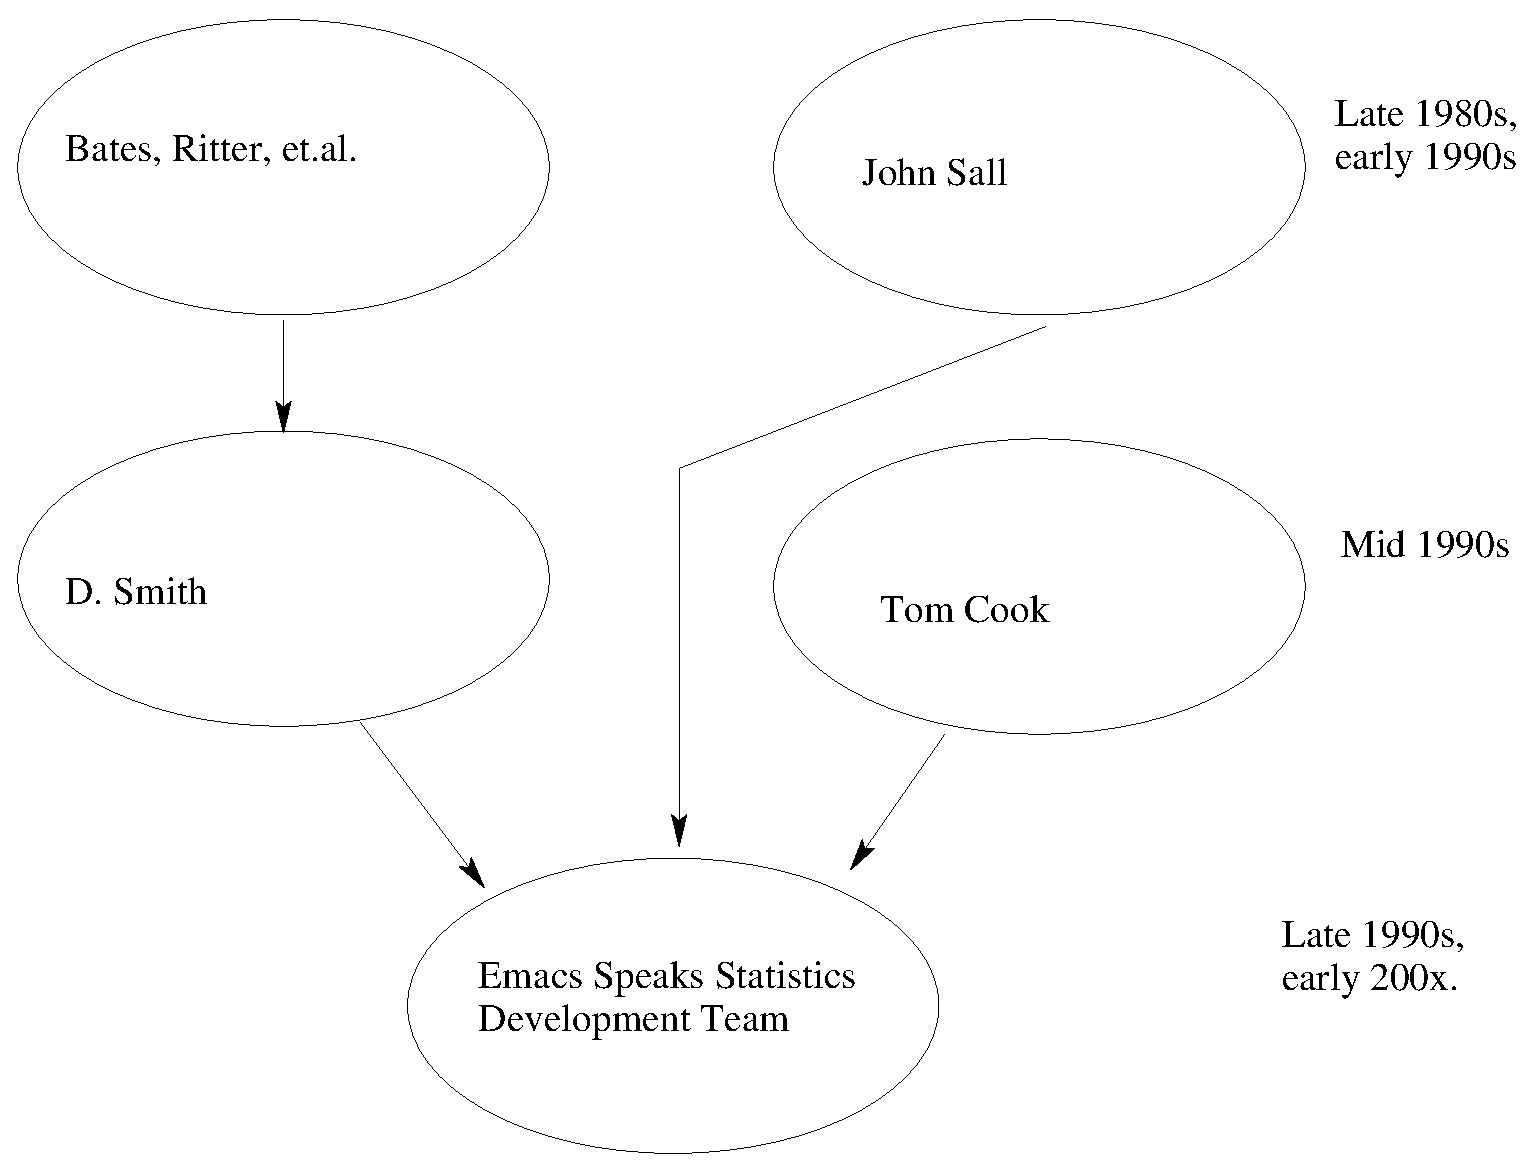
\includegraphics[height=3in,width=5.5in]{timeline} %% please use the eps.gz
%\fi
%  \caption{The history and timeline of ESS and its ancestors}
%  \label{fig:history}
%\end{figure}

\begin{table}[tbp]
  \centering
  \begin{tabular}{c ll c ll}
\hline
    Year  \\ 
\hline
         & \multicolumn{2}{c}{S-mode}       && \multicolumn{2}{c}{SAS-mode} \\ 
\cline{2-3} \cline{5-6}
    1989 & v.1 & (Emacs, Unix, S/S+)        &&  \\
    1990 &     &                            &&     & (Emacs, Unix, SAS editing) \\
    1991 & v.2 & (Emacs, Unix, S/S+)        && \\
    1993 & v.3 & (Emacs, Unix, S/S+)        && \\
    1994 & v.4 & (Emacs/XEmacs, Unix, S/S+) && v.1  & (Emacs, Unix, SAS batch) \\
    1995 & v.4.7 & (Emacs/XEmacs, Unix, S/S+/R) && v.2 & (Emacs/XEmacs, Unix, SAS batch) \\
    \cline{2-6}\\[-3.5ex]
    \cline{2-6}
         & \multicolumn{5}{c}{ESS (Emacs Speaks Statistics)} \\
    \cline{2-6} 
         &\multicolumn{2}{c}{Operating System} &&\multicolumn{2}{c}{Additional Functionality}\\
\cline{2-3} \cline{5-6}
    1997 & v.5.0 & (Emacs/XEmacs, Unix)         &&&  Stata, XLispStat, SAS interactive \\
    1998 & v.5.1.1 & (Emacs/XEmacs, Unix/Windows) &&&  S+elsewhere; Windows: S+/R\\
    1999 & v.5.1.10 & (Emacs/XEmacs, Unix/Windows/Mac) &&& SAS batch; Omegahat \\
    2001 & v.5.1.19 & (Emacs/XEmacs, Unix/Windows/Mac) &&& Unix/DOS: BUGS batch, Mac: R \\
%%    2002 & v.5.1.20 & (Emacs/XEmacs, Unix/Windows/Mac) &&& Unix/DOS: BUGS batch, Mac: R \\
%%    2002 & v.5.2 & (Emacs/XEmacs, Unix/Windows/Mac) &&& ? \\
\hline
  \end{tabular}
  \caption{History and Ancestors of ESS}
  \label{tab:timeline}
\end{table}

%% ESS originated as S-mode, which provided an interface for
%% programming and process control under GNU Emacs for \Splus\ version 3,
The history of ESS can be traced back to 1989, when S-mode was written
as an extension to GNU Emacs for editing S and \Splus\ files.  Version
1 was written by Doug Bates and Ed Kademan.  This was extended by
Frank Ritter and Mike Meyer to become version 2.  Meyer and David
Smith made further contributions which was version 3. David Smith
provided changes for version 4.
%%This was written by Doug Bates, Ed Kademan, Frank Ritter, and
%%Mike Meyer.  David Smith was the next primary maintainer, and his most
%%important contribution was to enhance the \Splus\
%%command-line interface and allow for control of multiple processes
%%simultaneously.  
In 1995, A.J. Rossini extended S-mode to support XEmacs.  Together
with extensions written by Martin M{\"a}chler, this
became version 4.5.  By 1996, S-mode was available for GNU Emacs and
XEmacs and supported S, \Splus, and R.  %Kurt Hornik was instrumental
%in enhancing support for R.
%%, in particular, providing \stexttt{Rd-mode}.

The other ancestor of ESS is SAS-mode, written by Tom Cook, which
began in 1994 and was partially based on GNU Emacs macros written by
John Sall.
%%\textbf{NEED TO GET DATES FROM AJR's ARCHIVE!?}.
Rossini extended SAS-mode to work with XEmacs in 1995, and this provided the
impetus for a single mode for statistical programming.
%%The extension to a language-independent, generic interface was further prompted
%%by the success of R and the desire for more complete R support.
This led to a merger of SAS-mode and S-mode along with changes
to accommodate multiple languages in a flexible way.  The product of this
marriage was called ESS version 5.

During 1996 and 1997, Richard M. Heiberger designed ``inferior'' ESS for \SAS.
At the same time, SAS-mode was further integrated into ESS.

In 1997, more changes were made to facilitate
%% the grand redesign of the internals occurred, where by a generic
%% means for
support for additional statistical languages like \Stata\ and \XLispStat.

Most of the work, until 1998, was for Unix statistics packages that
used the standard-input/standard-output model of inter-process
communication for both the command-line interface and batch file
processing.  ESS could not communicate with Windows versions of
statistical packages that did not use the
standard-input/standard-output model.  This hurdle fell in 1998 when
Brian Ripley demonstrated how ESS could use the Windows Dynamic Data
Exchange (DDE) protocol as an interface.  A variant of this was
incorporated soon after into ESS.
%  Based on this work, Heiberger provided interactive
%interfaces for Windows versions of \Splus.

%In 1998, Rodney Sparapani designed \SAS\ batch file processing for ESS
%on Unix, Windows and Mac.  In 1999 and 2000, Sparapani and Heiberger
%continually enhanced \SAS\ support. 
%In 2001 and 2002, they designed and implemented ESS-elsewhere for \SAS.  

%In 2001, Sparapani added BUGS batch file processing for ESS.

This history is summarized in Table \ref{tab:timeline}.

%\begin{Comment}
%Rich: see my discussion of ESS-elsewhere terminology.

%What is the behavior for remote SAS that is new for 2002?

%Rodney: SAS batch now works and Kermit was added as a method of transfer.
%\end{Comment}
%ESS-elsewhere provides interactive and batch processing
%with \SAS\ running on a remote machine that is accessed over a
%network.  This provides a powerful development environment for \SAS.

%%This
%%includes support for syntax highlighting and template-based source file
%%generation that provides the capability of specifying all the necessary
%%parameters for a BUGS batch run in a single file.

%%\section{Extensions}
%%\label{sec:extensions}

%%There are two active areas of extensions for user environments.  One
%%is to enhance the capabilities of the IDE for statistical practice;
%%this includes implementing such common IDE features as object
%%browsers, tool-tips, and interfacing cleaning.  The other is to target
%%appropriate potentially useful programming methodologies for transfer
%%to statistical practice.
%%
%%Literate Programming methodologies \citep{Knuth:1992,NRamsey:1994} are
%%a natural fit for statistical practice.  We refer to the application
%%to statistical analysis as Literate Statistical Practice
%%\citep{rossini:dsc:2001}.  The tools used are Noweb
%%\citep{NRamsey:1994} and either \LaTeX, \textsc{html}, or \textsc{xml}
%%for documenting and explaining the analysis.  This approach to
%%programming encourages the use of a literary documentation style to
%%explain the programming code for the data analysis.  The program can
%%then be extracted from the documentation text for realizing the
%%statistical analysis.

%future enhancement perhaps
%ESS provides the same ESS-elsewhere support for BUGS batch
%that it does for \SAS\ batch (see above).

Important extensions which should be implemented in future
versions include class browsers, analysis templates, tool-tips, and
similar features.  Class browsers can be thought of as a tree or
outline for presenting datasets, variables and functions in the
context of what they represent; this allows for rapid and appropriate
inspection.  Analysis templates would allow statistics centers and
groups to provide standardized templates for initiating an analysis.
%%While most IDE features have been developed for object-oriented
%%languages, the above also can apply to non-object oriented
%%programming.

%ESS is one of the first  Rapid Application Development (RAD)
%environments intended for statisticians.  It provides

\section{Conclusion}

ESS provides 
an enhanced, powerful interface for efficient interactive data
analysis and statistical programming.  
It allows the user complete control over the communications among the
files in which the analysis is specified, the statistical process doing
the computation, and the output.  Because all are within the same programming
environment, and therefore are accessed with the same
editing and searching concepts and keystrokes, user efficiency is increased.
It is completely customizable
to satisfy individual desires for interface styles as well as being
extensible to additional statistical languages and analysis packages.



\bibliographystyle{plainnat}
%\pdfbookmark[1]{References}{section.7}
\addcontentsline {toc}{section}{\numberline {}References}
\bibliography{essJCGSv2}

\clearpage

\appendix 
\section{Appendix: ESS Resources on the Internet}
\addcontentsline {toc}{section}{\numberline {}ESS Resources on the Internet}
\label{sec:access}

\paragraph{Latest Version.}

ESS is constantly in flux.  New versions of statistical
packages, Emacs and operating systems require new releases of ESS to
support them.  The latest stable version of ESS can be found on the web at
\url{http://software.biostat.washington.edu/statsoft/ess/}.  To get help
with problems, send e-mail to \url{ess-help@stat.math.ethz.ch}.
The latest development, hence unstable, version can be obtained by
anonymous CVS.  First type:

\stexttt{cvs -d
  :pserver:anoncvs@software.biostat.washington.edu:/var/anoncvs login}
  
You will be prompted for a password which is ``\stexttt{anoncvs}''.
Then type:

\stexttt{cvs -d
  :pserver:anoncvs@software.biostat.washington.edu:/var/anoncvs co
  ess}

\paragraph{Additional documentation.} 

An expanded version of the present paper is in \citep{RMHHS:2001}.  A
general introduction and usage instructions can be found in
\citep{heiberger:dsc:2001}; in addition, one which is more focused on
SAS can be found in \citep{heiberger:philasugi:2001}.  The
documentation that comes with ESS provides details of its
implementation as well as examples of its use.


\end{document}


%%% Local Variables:
%%% mode: latex
%%% TeX-master: t
%%% End:
